\section{Use cases: given a metabolic model...}
\label{section:use-cases}

La figura \footnote{aggiungere qui una figura che rappresenta gli use
  case in stile overview} riassume tutti i casi d'uso che abbiamo
implementato nella libreria. La notazione utilizzata \`e quella
offerta dal linguaggio \emph{UML}, limitandoci ai "costrutti" pi\`u
semplici per favorire la comprensione.

In questa sezione descriveremo i casi d'uso che vogliamo implementare
e, per ognuno di essi, mostreremo i risultati della realizzazione.

Come suggerisce il titolo di questa sezione, tutti i successivi use
case lavorano su un modello metabolico, sul quale vengono effettuate
le trasformazioni che andiamo a dettagliare. Inoltre, come il lettore
capir\`a nelle prossime righe, ogni use case pu\`o essere messo in
corrispondenza con il concetto di filtro. Questa associazione
porter\`a alla naturale astrazione che costituir\`a l'architettura
della nostra libreria.

\subsection{...build a model \emph{story-ready}}
L'operazione fondamentale a cui siamo interessati \`e poter manipolare
un modello metabolico, codificandolo con un sistema di oggetti che
permetta di applicare i concetti espressi in \footnote{aggiungere qui
  riferimento bibliografico all'articolo Crescenzi-Marino}.

Questo requisito precede tutti gli altri, in quanto questi suppongono
che il modello che vogliamo studiare sia gi\`a stato codificato nel
nostro modello dati.

Non possiamo dare nessun oggetto che sia la rappresentazione di questo
use case, in quanto la miglior rappresentazione del risultato della
sua esecuzione \`e un insieme di oggetti Java, di cui evitiamo di
riportare la rappresentazione testuale fornita dal metodo
\emph{toString()}.

\subsection{...represent it in \emph{black \& white}}
\label{subsection:represent-it-in-black-and-white}
Questo use case cattura il requisito di costruire un documento
interpretabile dai motori di renderizzazione offerti dalla libreria
\emph{graphviz}, rappresentando i nodi sorgenti e nodi pozzi con un
cerchio completamente riempito (\emph{black nodes}), mentre i nodi che
non sono ne sorgente ne pozzi con un cerchio vuoto (\emph{white
  nodes}).
\begin{figure}
  \centering
  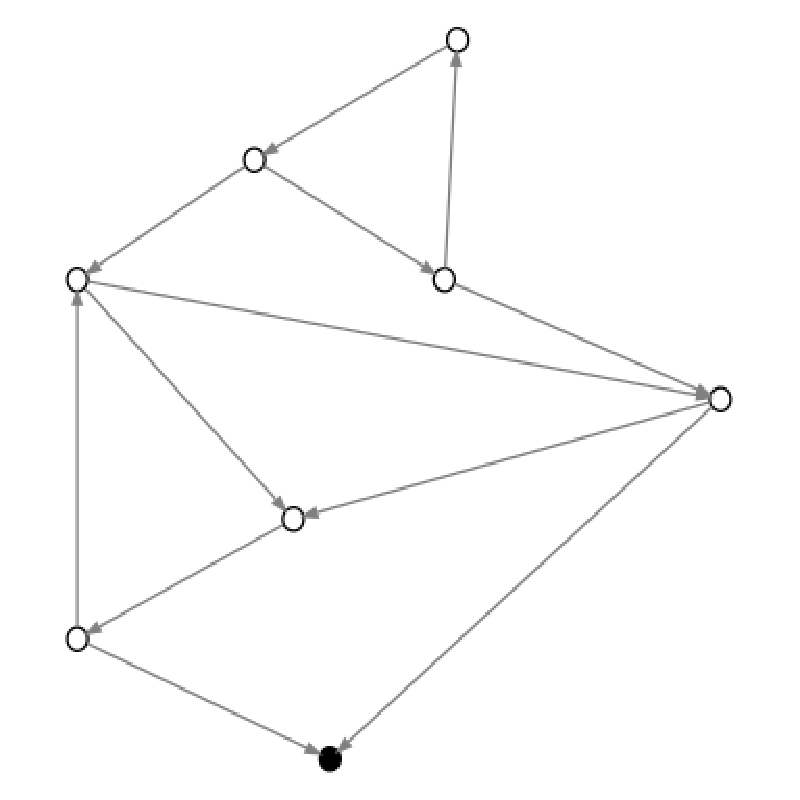
\includegraphics[scale=0.8]{images/applicationOfPrinterPipeFilterOnTarjanModel-phase-PrinterPipeFilter-level-0.eps}
  \caption{simple black \& white graph}
  \label{fig:simple-black-and-white}
\end{figure}

La figura \ref{fig:simple-black-and-white} riporta la rappresentazione
di un modello metabolico dopo esser stato codificato nel nostro
modello dati.

Questo use-case non ha restituisce nessuna trasformazione del grafo in
input, pertanto si limita a restituire il grafo originale.

\subsection{...apply a \emph{DFS search} and build its tree}
Questo use case cattura il requisito di applicare un ricerca
\emph{DFS} al grafo in input.

Il risultato prodotto da questo use-case \`e la foresta di alberi
\emph{DFS}, i cui archi sono un sottoinsieme dell'insieme di archi del
grafo originale visitati durante la computazione.

Inoltre, siamo interessati ad associare, per ogni vertice, una coppia
di interi che indica il momento in cui la visita esplora un vertice e
quando l'esplorazione del vicinato di tale vertice viene
completata. Queste informazioni possono risultare molto utili in fase
di studio del grafo; abbiamo ripreso questo spunto da
\footnote{aggiungere qui riferimento bibliografico a Algorithms}.

Vediamo i risultati di una sua esecuzione: la figura
\ref{fig:before-applying-dfs-search} riporta il grafo originale di
partenza, preso da \footnote{aggiungere qui riferimento bibliografico
  al volume di Papadimitriou Algorithms}:
\begin{figure}
  \centering
  
\includegraphics{images/OnePipingLevelUnitTest_Printer_DFS_PrinterPipe_Papadimitriou-phase-PrinterPipeFilter-level-0.eps}
  \caption{Before applying DFS search}
  \label{fig:before-applying-dfs-search}
\end{figure}
applicando la ricerca \emph{DFS} a tale grafo otteniamo la foresta di
alberi \emph{DFS}, riportata in figura \ref{fig:dfs-forest}, dopo aver
composto a questo use-case il precedente
\ref{subsection:represent-it-in-black-and-white}.
\begin{figure}
  \centering
  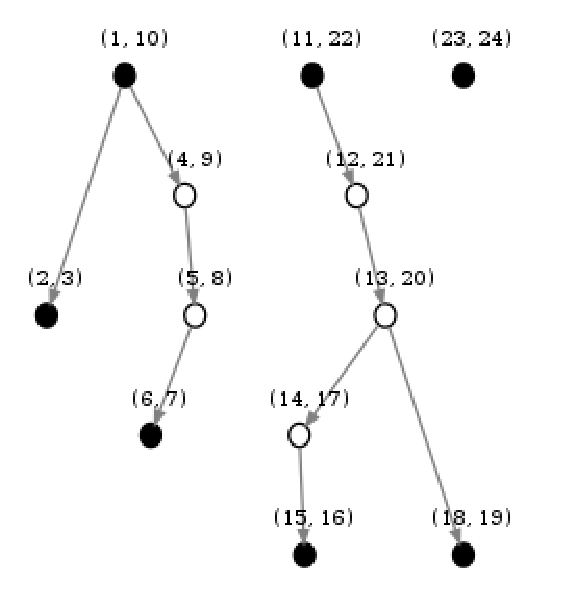
\includegraphics{images/OnePipingLevelUnitTest_Printer_DFS_PrinterPipe_Papadimitriou-phase-PrinterPipeFilter-level-2.eps}
  \caption{DFS forest}
  \label{fig:dfs-forest}
\end{figure}

\subsection{...apply the \emph{Tarjan algorithm} and build the
  minimized graph}
\label{subsection:use-case-tarjan}
Questo use case cattura il requisito di applicare l'algoritmo di
Tarjan per la ricerca delle componenti fortemente connesse al grafo di
input.

Il risultato prodotto da questo use-case \`e un grafo che ha
come nodi le componenti fortemente connesse e come archi la relazione
di vicinato tra le componenti.

Inoltre, siamo interessati ad associare, per ogni vertice, un intero
che indica la cardinalit\`a della componente fortemente connessa che
esso rappresenta.

Vediamo i risultati di una sua esecuzione: la figura
\ref{fig:before-applying-tarjan} riporta il grafo originale di
partenza, preso da \footnote{aggiungere qui riferimento bibliografico
  al volume di Crescenzi sulle strutture dati}:
\begin{figure}
  \centering
  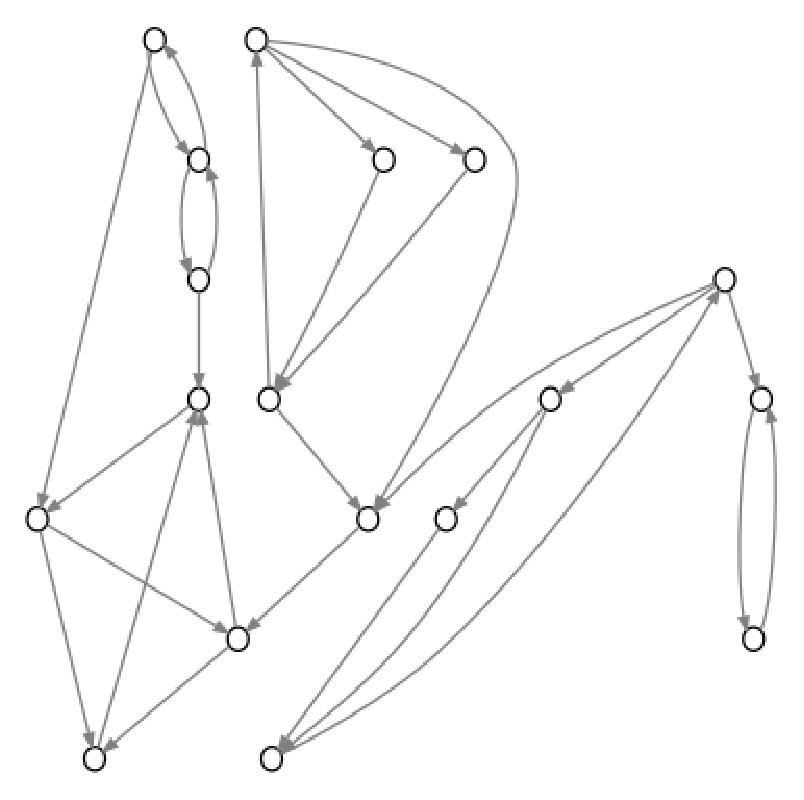
\includegraphics{images/OnePipingLevelUnitTest_Printer_DFS_PrinterPipe_Crescenzi-phase-PrinterPipeFilter-level-0.eps}
  \caption{Before applying Tarjan algorithm}
  \label{fig:before-applying-tarjan}
\end{figure}
applicando l'algoritmo di Tarjan a tale grafo otteniamo il grafo
minimizzato, riportato in figura \ref{fig:tarjan-output}, dopo aver
composto a questo use-case il precedente
\ref{subsection:represent-it-in-black-and-white}.
\begin{figure}
  \centering
  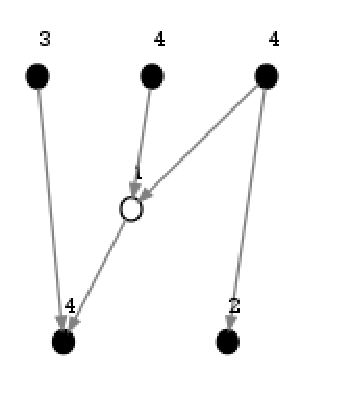
\includegraphics{images/OnePipingLevelUnitTest_Printer_DFS_PrinterPipe_Crescenzi-phase-PrinterPipeFilter-level-2.eps}
  \caption{Graph after Tarjan minimization}
  \label{fig:tarjan-output}
\end{figure}

\subsection{...represent it in \emph{plain text} tabular}
Questo use case cattura il requisito di rappresentare il grafo in
input in formato testuale, usando uno schema tabellare.

Il \emph{side-effect} prodotto da questo use-case \`e collezionare le
informazioni richieste visitando il grafo e scriverle in un file
dedicato.

Inoltre, per comodit\`a, vogliamo comporre pi\`u di un use-case ed
avere le informazioni relative ai grafi intermedi inserite nello
stesso documento.

Vediamo i risultati di una sua esecuzione, allegando un documento
prodotto:
\begin{lstlisting}
phase-PlainTextStatsPipeFilter-level-2
NOfVertices: 1
	NOfComponents:	206
	NOfEdges:	183
	NOfSources:	108
	NOfSinks:	96
	NOfWhites:	2

NOfVertices: 2
	NOfComponents:	9
	NOfEdges:	1
	NOfSources:	1
	NOfSinks:	8
	NOfWhites:	0

NOfVertices: 3
	NOfComponents:	5
	NOfEdges:	0
	NOfSources:	0
	NOfSinks:	5
	NOfWhites:	0

NOfVertices: 4
	NOfComponents:	1
	NOfEdges:	0
	NOfSources:	0
	NOfSinks:	1
	NOfWhites:	0

NOfVertices: 396
	NOfComponents:	1
	NOfEdges:	89
	NOfSources:	0
	NOfSinks:	0
	NOfWhites:	1

phase-PlainTextStatsPipeFilter-level-0
	NOfVertices:	639
	NOfEdges:	2209
	NOfSources:	108
	NOfSinks:	95
	NOfWhites:	436

\end{lstlisting}
Questo output necessita di alcune spiegazioni. Quello riportato \`e il
documento che viene generato da questo use-case, collezionando in un
primo momento le informazioni sul grafo originale (riportate sotto
l'etichetta \emph{phase-PlainTextStatsPipeFilter-level-0}) e in un
secondo momento, dopo aver applicato l'algoritmo di Tarjan, le
informazioni sul grafo minimizzato (riportate sotto l'etichetta
\emph{phase-PlainTextStatsPipeFilter-level-2}).

Come si nota i formati delle rappresentazioni tabulari sono vicini ma
non identici.

Le informazioni raccolte dopo il primo passo hanno la seguente
semantica; sia:
\begin{lstlisting}
phase-identifier
	NOfVertices:	v
	NOfEdges:	e
	NOfSources:	s
	NOfSinks:	d
	NOfWhites:	w
\end{lstlisting}
allora il grafo in input $G = (V, E)$, al passo
\emph{phase-identifier}, \`e tale che $|E| = e$ e $|V| = v$, di cui
$s$ vertici sono sorgenti, $d$ vertici sono pozzi e $w (= v -s -d)$
sono intermedi.

Definiamo adesso la semanrica associata alle informazioni collezionate
per il secondo passo. Come si pu\`o notare, queste informazioni
ripetono uno schema, del quale \`e sufficiente dare la semantica,
quante volte \`e necessario per elencare tutti i dati raccolti. Sia
dato il \emph{building-block}:
\begin{lstlisting}
NOfVertices: v
	NOfComponents:	c
	NOfEdges:	e
	NOfSources:	s
	NOfSinks:	d
	NOfWhites:	w  
\end{lstlisting}
allora nel grafo minimizzato esistono $c$ componenti fortemente
connesse, ognuna delle quali raggruppa $v$ vertici. Esistono $e$ archi
uscenti in totale dalle $c$ componenti e queste sono partizionate in
$s$ componenti sorgenti, $d$ componenti pozzo e $w$ componenti
intermedie.

Come abbiamo detto ad inizio sezione, questo use-case non trasforma il
grafo in input, anzi possiamo \`e ortogonale ed una intera
composizione di use-case in quanto, elencando i dati raccolti per ogni
specifico \emph{phase-identifier}, non ha dipendenze da ognuno di
essi.

\subsection{...\emph{collapse} its source to manage complexity}
Questo use case cattura il requisito di eliminare tutti i vertici
sorgenti contenuti nel grafo in input, introducendo al loro posto un
nuovo vertice sorgente, tale che il suo vicinato sia uguale all'unione
dei vicinati dei vertici rimossi.

Vediamo i risultati di una sua esecuzione, applicando la
minimizzazione al grafo di input, dopo aver composto a questo use-case
il precedente \ref{subsection:represent-it-in-black-and-white}:
\begin{lstlisting}
phase-PlainTextStatsPipeFilter-level-1
	NOfVertices:	386
	NOfEdges:	1339
	NOfSources:	1
	NOfSinks:	85
	NOfWhites:	300
\end{lstlisting}
Come si vede dalle informazioni riportate, il nuovo grafo, input per
successive computazioni, ha un solo vertice sorgente.

\subsection{...\emph{inspect} its connected components and \emph{show}
  them in a simple GUI}
\label{subsection:use-case-result-viewer}
Questo use case cattura il requisito di rappresentare informazioni
relative alle componenti fortemente connesse attraverso una semplice
GUI utilizzando il framework \emph{SWING}.

In realt\`a quello che ci piacerebbe costruire \`e un visualizzatore
di strutture dati, costruite appositamente per contenere le
informazioni di interesse, senza essere dipendenti dal risultato di
una computazione appena conclusa. Ovvero, vorremmo serializzare tale
struttura dati in una path del file system e poterla visualizzare
successivamente. Questo secondo noi \`e un approccio pi\`u modulare in
quanto permette di creare strutture dati e poterle scambiare,
utilizzando la maschera come semplice \emph{render}, anche se non
abbiamo generato noi stessi la serializzazione delle informazioni.

Inoltre siamo interessati a condurre la nostra indagine restringendosi
non solo ad un modello (e quindi ad un solo grafo), bensi vorremmo
analizzare un insieme di modelli affinch\`e sia possibile studiare in
che tipo di \emph{strongly connected components} ogni \emph{species}
incontrata appare.

\begin{figure}
  \centering
  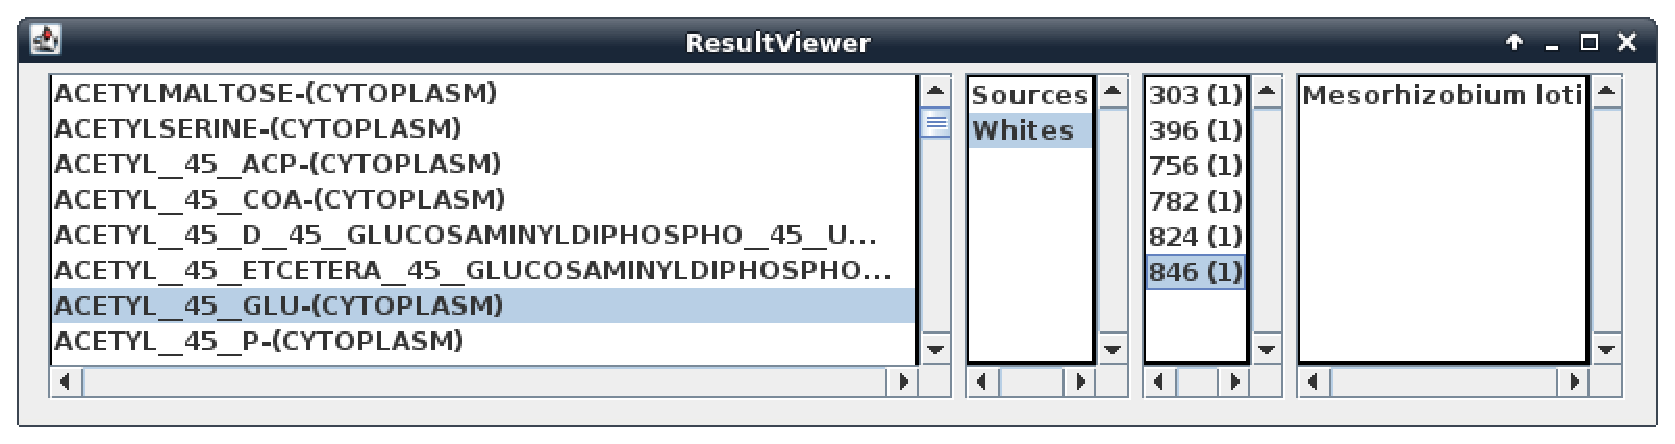
\includegraphics[scale=.5,
  angle=90]{images/ResultViewer-execution.eps}
  \caption{Result Viewer for strongly connected components}
  \label{fig:result-viewer-scc}
\end{figure}
La figura \ref{fig:result-viewer-scc} riporta uno screenshot, diamo
adesso la semantica alle informazioni rappresentate nella maschera.

Il frame contiene i seguenti componenti, che andiamo a descrivere
seguendo l'ordine da sinistra verso destra e dall'alto verso il basso:
\begin{itemize}
\item una tabella dove vengono elencati tutti i modelli che sono stati
  oggetto di indagine. Per ogni modello si associano tre triple $(c,
  v)$ per tre colonne, ognuna rappresentante una tipologia di vertice
  (\emph{sources, whites, sinks}). Se una coppia $c, v$ appartiene
  alla riga del modello $m$ e alla colonna $whites$ per esempio,
  allora significa che nel modello $m$ esistono $c$ strongly connected
  components di tipo $whites$, le quali contengono in totale $m$
  vertici (che di conseguenza hanno pure loro il ruolo di $whites$).
\item una \emph{list-box} nella quale sono riportate delle
  informazioni relative alle \emph{species}. Ogni entry raggruppa le
  \emph{species} in base ai ruoli (ovvero in base alla tipologia di
  vertice) che hanno in tutti i modelli analizzati. 

  Inoltre si calcola anche una loro frequenza in percentuale per avere
  un raffronto immediato riguardo alla predominanza dei ruoli svolti:
  si considerano tutte le possibili combinazioni dell'insieme
  ${sources, whites, sinks}$, escludendo l'insieme vuoto.
\item nella successiva \emph{list-box} vengono elencate tutte le
  \emph{species} contenute in almeno uno dei modelli oggetto
  dell'indagine. Ogni \emph{species} \`e codificata con una stringa
  composta dall'identificatore e, tra parantesi tonde, il nomde del
  compartimento in cui risiede.
\item cliccando su una \emph{species} $s$, nella successiva
  \emph{list-box} vengono elencati i tipi delle \emph{strongly
    connected components} che contengono la \emph{species} $s$.
\item cliccando su una tipologia $t$ di \emph{strongly connected
    components}, nella successiva \emph{list-box} vengono elencate le
  cardinalit\`a delle \emph{strongly connected components} che
  contengono la \emph{species} $s$ e sono di tipologia $t$. Ad ogni
  cardinalit\`a si concatena un numero intero che indica la
  cardinalit\`a dell'insieme rappresentato nell'ultima
  \emph{list-box}, che andiamo a descrivere.
\item cliccando su una cardinalit\`a $c$, nell'ultima \emph{list-box}
  vengono elencati i modelli, la cui applicazione dell'algoritmo di
  Tarjan, ha prodotto un grafo in cui esiste una \emph{strongly
    connected component} tale che contiene la \emph{species} $s$, \`e
  di tipo $t$ ed ha una cardinalit\`a $c$.
\end{itemize}

Non solo le ultime quattro \emph{list-box} sono contestualmente
correlate, ma anche la tabella e la \emph{list-box} con le
informazioni per tipologia di vertice lo sono. In particolare,
selezionando nella tabella una o pi\`u righe, nella \emph{list-box}
\`e possibile avere le informazioni riguardo alle species contenute
nei modelli selezionati. Se la selezione \`e vuota, allora le
informazioni sono relative a tutti i modelli.

Inoltre abbiamo esteso queste correlazioni anche tra il percorso
selezionato nelle ultime quattro \emph{list-box} e la tabella (e di
conseguenza alla prima \emph{list-box}). Selezionando una
\emph{species} dalla seconda \emph{list-box} vengono selezionati in
automatico nella tabella tutti i modelli che la contengono e, come
spiegato nel paragrafo precedente, anche la \emph{list-box} contenente
le informazioni per tipologia di vertice verr\`a aggiornata di
conseguenza.

Se si raffina il percorso, ad esempio scegliendo la tipologia di
vertice e la cardinalit\`a nelle rispettive \emph{list-box}, viene
raffinata la selezione nella tabella dei modelli.

\subsection{...ignore it and process \emph{your own graph}}
Nelle precedenti sezioni abbiamo sempre assunto di lavorare su un
modello metabolico (\emph{given a metabolic model...}), ma niente ci
vieta di poter utilizzare la libreria su un grafo che costruiamo
direttamente utilizzando oggetti del nostro modello dati.

Questo rende la libreria non strettamente legata ai concetti nel campo
della biologia e, in particolare, delle reti metaboliche, restando
invece aperta ad utilizzi nel campo della teoria dei grafi (in
realt\`a il grafo riportato in figura \ref{fig:simple-black-and-white}
non \`e altro che il grafo utilizzato da Tarjan nel suo articolo
\footnote{aggiungere qui riferimento bibliografico all'articolo di
  Tarjan sull'algoritmo per le componenti fortemente connesse}).


